\section{Dimensional analysis}
\subsection{Dimensions and units}
Many problems in dynamics involve 3 basic dimensional equantities:
\begin{align*}
    {\color{blue}L} \quad &\text{length},\\ 
    {\color{blue}M} \quad &\text{mass},\\ 
    {\color{blue}T} \quad &\text{time}.
\end{align*}
Dimensions of some quantity $ [x] $ can be expressed in terms of $L,M,T$.

\begin{example}
    $ [\text{density}]=ML^{-3} $, $ [\text{force}]=MLT^{-2} $.
\end{example}
\begin{note}
    Only power law functions of $M,L,T$ are allowed. e.g. do not allow $e^x$ with $x$ dimensional, since it is meaningless to add things with different dimensions.
\end{note}

We can introduce \textbf{units} for $L,M,T$. e.g. the SI units give $ \mathrm{m} $ for $L$, $ \mathrm{kg} $ for $M$, and $\mathrm{s}$ for $T$. Many other physical quantities can be formed out of these units.
\begin{example}
    $ [G]=M^{-1}L^3T^{-2} $ and has unit $ \mathrm{m}^3 \mathrm{kg}^{-1}\mathrm{s}^{-2} $.
\end{example}

\begin{law}
    Dynamical/Physical equations must work for any consistent choice of units.
\end{law}

\subsection{Scaling}

Suppose that a dimensional quantity $ Y $ depends on a set of dimensional quantities
\[
    \{X_1,X_2,\dots,X_n\}.
\]
Let $ [Y]=L^aM^bT^c $, and $ [X_i]=L^{a_i}M^{b_i}T^{c_i} $ for $i=1,\dots,n$. 

If $n\le 3$, then 
\[
    Y = C X_1^{p_1}X_2^{p_2}X_3^{p_3}
\]
and $p_i$ can be determined by balancing dimensions. Hence
\[
    \begin{pmatrix}
        a \\ b \\ c
    \end{pmatrix}=\begin{pmatrix}
        a_1 & a_2 & a_3 \\
        b_1 & b_2 & b_3 \\
        c_1 & c_2 & c_3 \\
    \end{pmatrix}\begin{pmatrix}
        p_1 \\ p_2 \\ p_3
    \end{pmatrix},
\]
with a unique solution for $p_i$ if dimensions of $X_i$ are independent.

If $n>3$ then $X_i$ are \textit{not} dimensionally independent\footnote{Since there are only 3 dimensions}. Wlog, choose $X_1,X_2,X_3$ that are dimensionally independent, and express the rest of the quantities as $n-3$ \textit{dimensionless} quantities $ \lambda_i $ such that 
\[
    \lambda_{i} = \frac{X_{i+3}}{X_1^{q_{i1}}X_2^{q_{i2}}X_3^{q_{i3}}},
\]
where $q_{ij}$ are chosen to balance dimensions. Hence 
\[
    Y=X_1^{p_1}X_2^{p_2}X_3^{p_3}C(\lambda_1,\lambda_2,\dots,\lambda_{n-3}),
\]
where $C$ is a dimensionless function of $ \lambda_i $. This is called the \textbf{Bridgeman's theorem}.

\begin{example}[Simple peldulum]\label{eg:simple pendulum}
    Consider a simple pendulum with length $l$ and initial horizontal displacement $d$. How does the period $p$ of the oscillator change with $m,l,d,g$?
    \begin{center}
        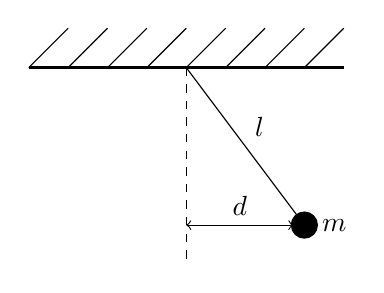
\begin{tikzpicture}
            \draw[thick] (-2,2) -- (2,2);
            \foreach \p in {-2,-1.5,...,1.5}
                \draw (\p,2) -- (\p+0.5,2.5);
            \draw[dashed] (0,2) -- (0,-0.5);
            \draw (0,2) -- (1.5,0) node[pos = 0.5, anchor = south west] {$l$} node[fill=black, draw=black, shape=circle] {} node[right] at (1.6,0) {$m$};
            \draw[<->] (0,0) -- (1.36,0) node[pos=0.5, above] {$d$};
        \end{tikzpicture}
    \end{center}
    Note that $ [p]=T, [m]=M, [g]=LT^{-2}, [l]=[d]=L $. Choose $m,g,l$ as independent quantities\footnote{$l$ is more suitable than $d$ since $l$ does not depend on initial displacement.}. Hence 
    \[
        p = f\left( \frac{d}{l} \right)m^{p_1}l^{p_2}g^{p_3} \Longrightarrow T=M^{p_1}L^{p_2+p_3}T^{-2p_3}.
    \]
    Balance dimensions gives $ p_1=0, p_2= 1/2, p_3=-1/2$, and thus 
    \[
        p = f\left( \frac{d}{l} \right) \sqrt{\frac{l}{g}}.
    \]
\end{example}
\begin{example}[Taylor's estimate of energy of the 1st atomic explosion]
    Let $ R(t) $ be the size of a fireball as a function of time. It has dimension $ L $. The density of air $\rho$ has dimensions $ ML^{-3} $ and the energy of explosion $E$ has dimensions $ ML^2T^{-2} $. We can write 
    \[
        R = C t^{\alpha}\rho^{\beta}E^{\gamma}\Longrightarrow L=L^{2\gamma-3\beta}M^{\beta+\gamma}T^{\alpha-2\gamma}.
    \]
    Hence $ \alpha=2/5 , \beta=-1/5,\gamma=1/5 $. Hence
    \[
        R(t)=C t^{2/5}\rho^{-1/5}E^{1/5} \Longrightarrow E = \frac{\rho R^5}{C^5 t^2}.
    \]
    Note that by measurement of the photographs of explosion,
    \[
        \frac{R^5}{t^2} \approx 6.7 \times 10^{13} \mathrm{m}^5 \mathrm{t}^{-2},\quad \rho \approx 1.25 \mathrm{kg} \mathrm{m}^{-3}.
    \]
    If $C\approx 1$ then $ E \approx 10^{14}J \approx 24 \times 10^{3} \text{ tonnes of TNT} $.
\end{example}